\documentclass[12pt,a4paper]{article}
\usepackage[utf8]{inputenc}
\usepackage[T1]{fontenc}
\usepackage{amsmath}
\usepackage{amsfonts}
\usepackage{amssymb}
\usepackage{amsthm}
\usepackage{graphicx}
\usepackage{subfigure}
\usepackage{float}
\newtheorem*{lemma}{Lemma}
\newtheorem*{theorem}{Theorem}
\newtheorem*{prf}{\textbf{Proof}}
\usepackage{caption}
\DeclareMathOperator{\n}{\nabla}
\DeclareMathOperator{\E}{\mathrm{E}}
\DeclareMathOperator{\xyz}{\textbf{numpy.random.normal()}}
\title{CS331-HW4-Lukang-Sun}
\begin{document}
	\maketitle
	\paragraph{p1.}
	\begin{theorem} 
	Assume $f$ is convex and L-smooth and $\mu-$convex. Define the gradient estimator
	$$
	g(x) \stackrel{\text { def }}{=} \mathcal{C}(\nabla f(x))
	$$
	where $\mathcal{C}: \mathbb{R}^{d} \rightarrow \mathbb{R}^{d}$ is a compression operator defined in problem 1. Then(AC-condition)
	\begin{equation}
		G(x, y) \leq 2 \underbrace{(2 \omega+1) L}_{A} D_{f}(x, y)+\underbrace{2 \omega\|\nabla f(y)\|^{2}+\delta}_{C(y)},
	\end{equation}
	and the iteration of CGD(Algorithm 11 in the lecture) satisfy
	\begin{equation}
		\E\left[||x^k-x^{\star}||^2\right]\leq (1-\gamma\mu)^k||x^0-x^{\star}||^2+\frac{\gamma (2\omega||\n f(x^{\star})||^2+\delta) }{\mu},
	\end{equation}
	where $0<\gamma\leq \frac{1}{A}$
	
	\end{theorem}

	\begin{proof}
	\begin{equation*}
		\begin{aligned}
			G(x,y)&\stackrel{\text{ref}}{=} \E\left[||g(x)-\nabla f(y)||^2\right]\\
					 &=\E\left[||g(x)-\ \n f(x)||^2\right]+||\n f(x)-\n f(y))||^2\\
					 &=\E\left[||\mathcal{C}(\n f(x))-\n f(x)||^2\right]+||\n f(x)-\n f(y)||^2\\
					 &=w||\n f(x)||^2+\delta+||\n f(x)-\n f(y)||^2\\
					 &=w||\n f(x)-\n f(y)+\n f(y)||^2+||\n f(x)-\n f(y)||^2+\delta\\
					 &=2w||\n f(x)=\n f(y)||^2+2w||\n f(y)||^2+||\n f(x)-\n f(y)||^2+\delta\\
					 &=(2w+1)||\n f(x)-\n f(y)||^2+2w||\n f(y)||^2+\delta\\
					 &=2(2w+1)LD_f(x,y)+2w||\n f(y)||^2+\delta,
		\end{aligned}
	\end{equation*}
	where in the last step we have used convexity and $L-$smoothness of $f$, this proves (1). (2) is a direct consequence of the AC-condition, where $A=(2\omega+1)L, C=2\omega||\n f(x^{\star})||^2+\delta.$
	
	\end{proof}
	\paragraph{p2.}
	In my experiments(see Figure\ref{img2}.), I set $d = 1, n = 10, \epsilon = 10^{-4},  f(x)=\frac{1}{ 10} \sum_{i=1}^{10} f_i(x), f_i(x) = \frac{1}{2}\left\|a_{i}^{} x-b_{i}\right\|_{2}^{2}$, $a = [2,4,6,3,2,9,6,7,11,45], b = [1,2,3,4,5,6,7,8,9,11]$, based on these information, we can get that $x_{\star} = 0.3343133137337253, \sigma_{\star}^2 = 3993.739347850591, \max_{i} L_i = 2025, L = \mu = 238.1. $I use Bernoulli compressor(I.I.D.) with $p=\left[0.1,0.2,0.3,0.4,0.5,0.6,0.7,0.8,0.9,1\right],$ so
	\newline $\omega+1=\left[10,5,3.3,2.5,2,1.67,1.43,1.25,1,11,1\right]$ , I sample 500 points in the last step to estimate $\mathrm{E}\left[||x_{\text{last step}}-x_{\star}||^2\right]$. From the experiment results, it quite match Lemma 51 in the lecture.
	\begin{figure}
		\centering
		\subfigure[ ]{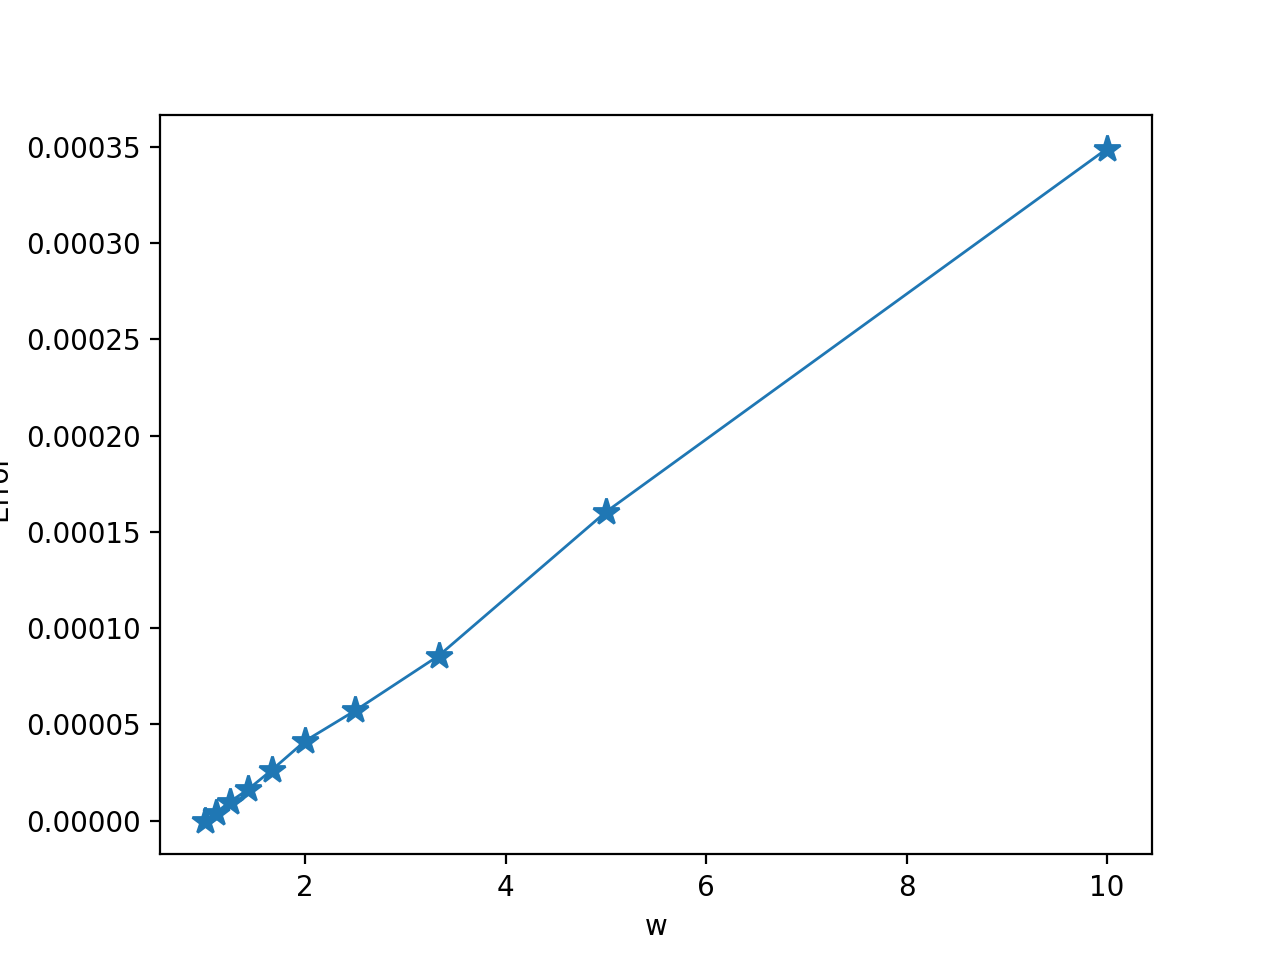
\includegraphics[width=6.7cm]{Figure_42.png}} 
		\subfigure[]{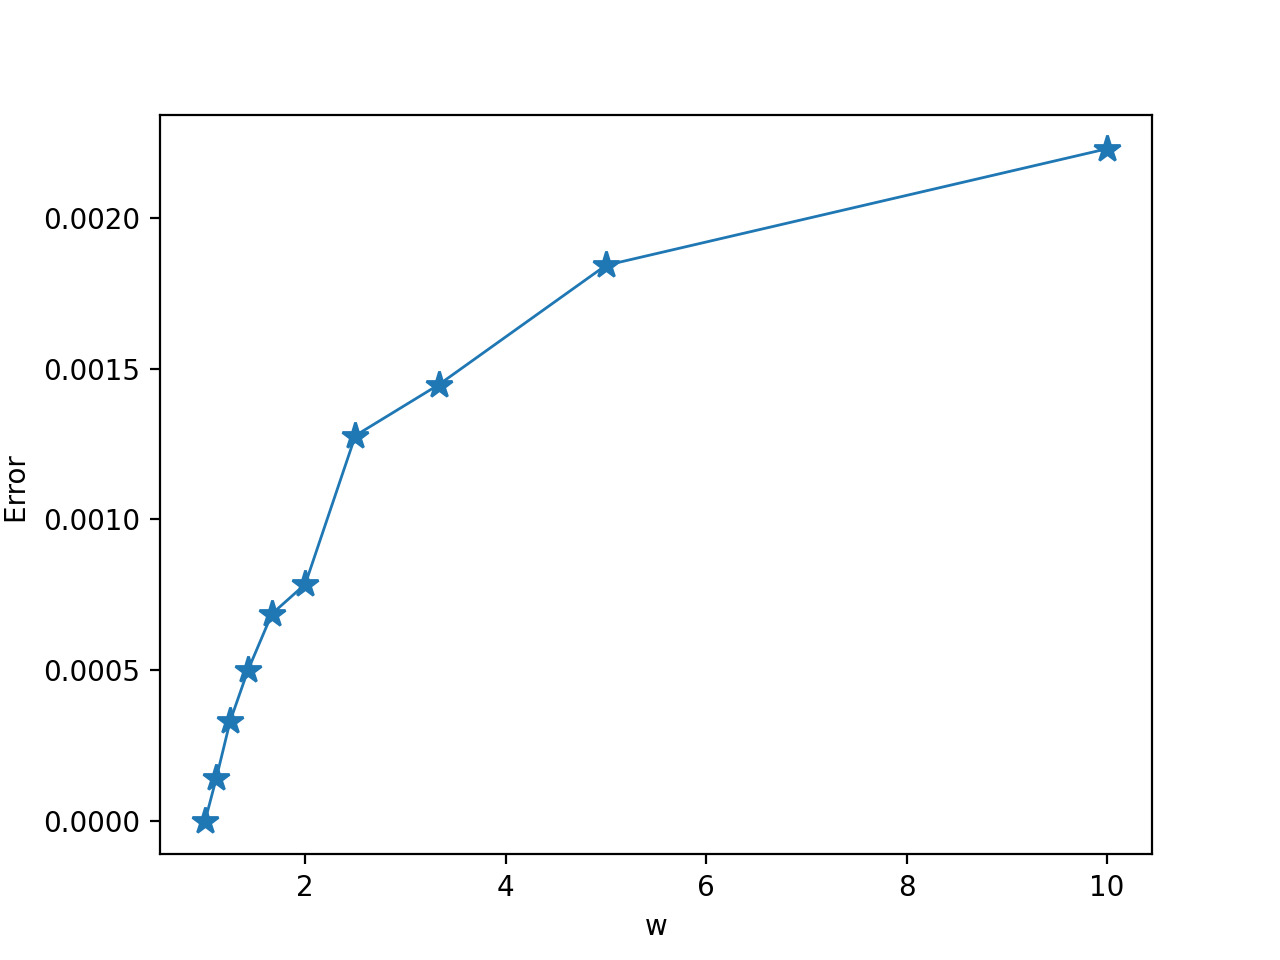
\includegraphics[width=6.7cm]{Figure_43.png}}
		\\ %换行
		
		
		\caption{  The horizontal axis is $\omega+1$, vertical axis is the error, you can see the trend that when $\omega$ gets bigger, the error will also gets bigger, this quite match the theoretical analysis. In picture (a), I use constant step size $\gamma=\frac{1}{22000}$, while in picture (b), I use step size $\gamma =\frac{1}{A}$, where $A = L+\frac{2w}{n}L_{max},\text{  where  }   n=10$.} %图片标题
		\label{img2}
	\end{figure}
	
	\paragraph{p3.}
	Let $\delta(\omega_1)$ uniformly chosen from $\left[-\epsilon,+\epsilon\right]$,  random matrix $A(\omega_1)$ and its entry $A(\omega_1)_{ij}$equals$1$, if $i=j$, equals $\delta(\omega_1)$if $i=j+1$, equals $-\delta(\omega_1)$ if $i=j-1$. Let $C(\omega_2)$ be drawn which independtly from $A(\omega_1)$ from random sparsification operator ensemble, then we construct the linear compression operator $K(\omega_1,\omega_2)=C(\omega_2)A(\omega_1)$. We can see random matrix$K$ is a small perturbation of  the sparsifier. We can prove that $\E\left[K(\omega_1,\omega_2)\right]=\boldsymbol{I}_d$, and $\E\left[K^{\top}K\right]$ exists(at least exists for small enough $\epsilon$). It is meaningful, since it acts just like sparsifier except add some noise to the non zero entry after sparsification. 
	
	
	
	\paragraph{p4.}
	for symmetry, 
	\begin{equation*}
		\mathrm{E}\left[\boldsymbol{C}^{\top} \boldsymbol{C}\right]^{\top}=\mathrm{E}\left[(\boldsymbol{C}^{\top} \boldsymbol{C})^{\top}\right]=\mathrm{E}\left[\boldsymbol{C}^{\top} \boldsymbol{C}\right],
	\end{equation*}
	for positive definiteness, choose any vector $x\in \mathbb{R}^d$, we have
	\begin{equation*}
		x^{\top}\mathrm{E}\left[\boldsymbol{C}^{\top} \boldsymbol{C}\right]x=\mathrm{E}\left[x^{\top}\boldsymbol{C}^{\top} \boldsymbol{C}x\right]\geq 0,
	\end{equation*}
	since $x^{\top}\boldsymbol{C}^{\top} \boldsymbol{C}x = ||\boldsymbol{C}x||_2^2\geq 0.$
	\paragraph{p5.}
	
	\begin{equation*}
		\begin{aligned}
		\lambda_{\text{max}}(\boldsymbol{P}^{1/2}\boldsymbol{L}\boldsymbol{P}^{1/2})	&=\max_{x}\frac{x^{\top}\boldsymbol{P}^{1/2}\boldsymbol{L}\boldsymbol{P}^{1/2}x}{x^{\top}\boldsymbol{P}x}\frac{x^{\top}\boldsymbol{P}x}{||x||^2}\\
		&\leq\max_{\boldsymbol{P}^{1/2}x}\frac{x^{\top}\boldsymbol{P}^{1/2}\boldsymbol{L}\boldsymbol{P}^{1/2}x}{x^{\top}\boldsymbol{P}x}\max_{x}\frac{x^{\top}\boldsymbol{P}x}{||x||^2}\\
		&\leq \lambda_{\text{max}}(\boldsymbol{L})\max_{x}\frac{x^{\top}\boldsymbol{P}x}{||x||^2}\\
		&\leq \lambda_{\text{max}}(\boldsymbol{L})\lambda_{\text{max}}(\boldsymbol{P}).
		\end{aligned}
	\end{equation*}
	( $\boldsymbol{P}$ should be $\boldsymbol{P}^{-1}$.)For the first inequality, I can not prove the general case. The first inequality is equivalent to 
	\begin{equation*}
		\max_{||x||^2_2\leq 1}\sum_{i,j}L_{i,j}\frac{P_{i,j}}{P_iP_j}x_ix_j\leq \max_{||x||^2_2\leq 1}\sum_{i,j}L_{i,j}\frac{P_i^{1/2}P_j^{1/2}}{P_iP_j}x_ix_j,
	\end{equation*}
where $P_{i,j}:=\sum_{S}P(S)1_{S}(i)1_{S}(j),P_{i}:=\sum_{S}P(S)1_{S}(i)$, we know $P_{i,j}\leq P_i^{1/2}P_j^{1/2}$, for any $(i,j)$. But for matrix $[P_{i,j}]$ whose entry is $P_{i,j}$ and matrix $[P_i^{1/2}P_j^{1/2}]$ whose entry is $P_i^{1/2}P_j^{1/2}$, we don't have $[P_{i,j}]\preccurlyeq[P_i^{1/2}P_j^{1/2}]$(we have $\lambda_{\max}([P_{i,j}])\leq\lambda_{\max}([P_i^{1/2}P_j^{1/2}])$, the purpose is to prove $\lambda_{\max}([P_{i,j}]\circ L)\leq\lambda_{\max}([P_i^{1/2}P_j^{1/2}]\circ L)$, where $L$ is semi positive definite.)
\newline
\textbf{Case one: $L$ has nonnegative entries(this include the case that L is diagonal.)} Choose $x$ such that $\lambda_{\max}(\mathrm{E}[C^{\top}LC])=\sum_{i,j}L_{i,j}\frac{P_{i,j}}{P_iP_j}x_ix_j$, then $\sum_{i,j}L_{i,j}\frac{P_{i,j}}{P_iP_j}x_ix_j\leq \sum_{i,j}L_{i,j}\frac{P_{i,j}}{P_iP_j}|x_i||x_j|\leq \sum_{i,j}L_{i,j}\frac{P_i^{1/2}P_j^{1/2}}{P_iP_j}|x_i||x_j|\leq  \max_{||x||^2_2\leq 1}\sum_{i,j}L_{i,j}\frac{P_i^{1/2}P_j^{1/2}}{P_iP_j}x_ix_j=\lambda_{\max }\mathrm{E}[P^{-1/2}LP^{-1/2}].$
\newline
\textbf{Case two: L has rank one.} In this case there is vector $\tilde{L}$, such that $L_{i,j}=\tilde{L}_i\tilde{L}_j$. Choose $x$ such that $\lambda_{\max}(\mathrm{E}[C^{\top}LC])=\sum_{i,j}\frac{P_{i,j}}{P_iP_j}\tilde{L}_ix_i\tilde{L}_jx_j$, then $\sum_{i,j}\frac{P_{i,j}}{P_iP_j}\tilde{L}_ix_i\tilde{L}_jx_j\leq \sum_{i,j}\frac{P_{i,j}}{P_iP_j}|\tilde{L}_ix_i||\tilde{L}_jx_j|\leq \sum_{i,j}\frac{P_i^{1/2}P_j^{1/2}}{P_iP_j}|\tilde{L}_ix_i||\tilde{L}_jx_j|\overset{\text{change sign of $x_i$ such that $\tilde{L}_ix_i$ nonnegative}}{\leq}  \max_{||x||^2_2{\leq} 1}\sum_{i,j}\frac{P_i^{1/2}P_j^{1/2}}{P_iP_j}\tilde{L}_ix_i\tilde{L}_jx_j=\lambda_{\max }\mathrm{E}[P^{-1/2}LP^{-1/2}].$
	\newline
	If $$\lambda_{\max }\left(\mathrm{E}\left[C_{S} LC_{S}\right]\right) \leq \lambda_{\max }\left(P^{-1 / 2} L P^{-1 / 2}\right) \leq \lambda_{\max }(L) \lambda_{\max }(P^{-1}),$$
	this means the step size for the third analysis can be at least as big as the second convergence analysis and in the second convergence analysis, the step size can be as big as  the the step size in the first convergence analysis. So the convergence rate for the third one is better than the second one, the second one is better than the first one.
	
	
	
\end{document}